\documentclass{resonance}
\usepackage[hidelinks]{hyperref}
\usepackage{xcolor}

\setlength{\fboxsep}{0pt}

\begin{document}

\title{Mathematical Simulations through Monte Carlo Methods}
\secondTitle{Fractal Trees and the Approximation of Pi}
\author{Akshansh Bhanjana - Aryan Gupta}

\maketitle
\authorIntro{\includegraphics[width=2cm]{akshansh}\\
Akshansh Bhanjana is a sophomore at Cluster Innovation Centre,
University of Delhi, currently majoring in Information Technology and Mathematical Innovations.\\
\authorIntro{\includegraphics[width=2cm]{aryan}\\
Aryan Gupta is a student at the University of Delhi,
with interests in Machine Learning, Robotics, and Computational Biology.}}

\begin{abstract}
Algorithms involving Monte Carlo Methods are comparatively scalable. They see a lot of usage in physical systems. This method can reduce complex models to simpler events, which can be simulated with ease. This paper involves simulations of two such mathematical phenomena: Estimating the Value of Pi, and Fractal Trees.
\end{abstract}

\monthyear{June 2020}
\artNature{GENERAL ARTICLE}


\section*{Introduction}
In probability, we find various situations where an analytical solution cannot be calculated directly. This calculation may be difficult due to various reasons such as many random variables, disturbances (noise) in the observations, etc.

In such a situation, it's possible to find probability distributions involving random variables using simulations.

Monte Carlo Methods / Experiments are algorithmic simulations which depend on repeating random sampling to get analytical results.\textsuperscript{[1]} They allow significance in the risks of quantitative analysis. This concept uses randomness to find probability distributions.

This technique is quite effective; it was used to make the atom bomb.

The three basic use cases of Monte Carlo are:
\begin{itemize}
    \item \textbf{estimating} Probability Distribution of a function
    \item \textbf{approximating} mean, variance, or other such quantities
    \item \textbf{optimizing} functions, i.e. maximizing / minimizing functions
\end{itemize}

\subsection*{Fractals}

\authorIntro{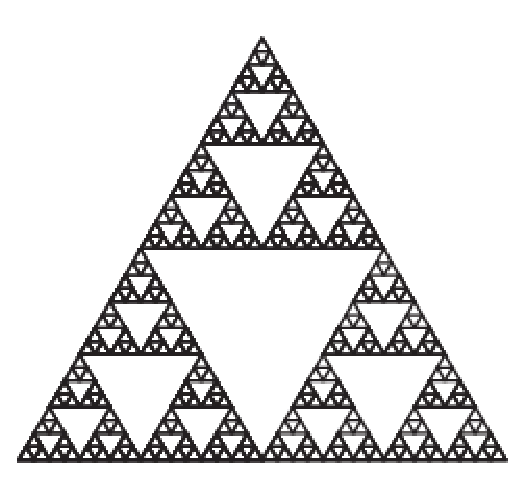
\includegraphics[width=3cm]{fractal_1}\\
\authorIntro{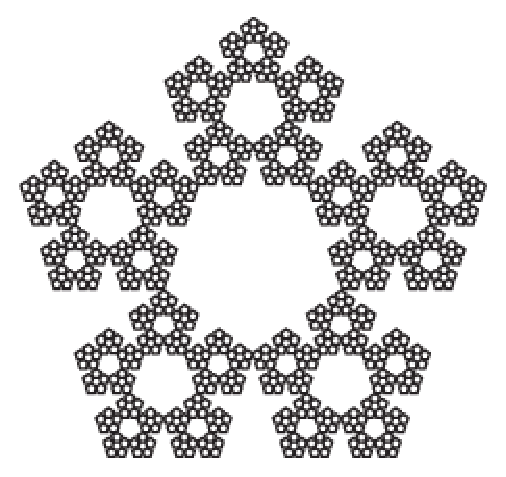
\includegraphics[width=3cm]{fractal_2}\\
\authorIntro{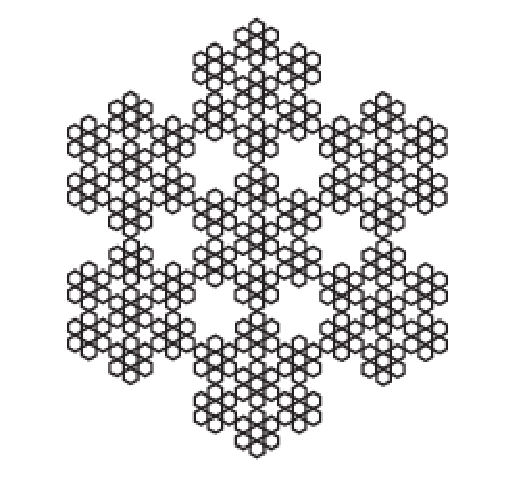
\includegraphics[width=3cm]{fractal_3}\\
\authorIntro{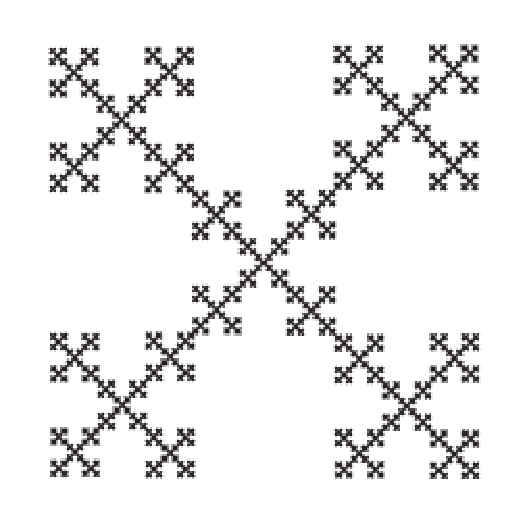
\includegraphics[width=3cm]{fractal_4}\\
Pictures taken from \textcolor{blue}{\url{https://researchgate.net}}}}}}

A fractal is "a rough or fragmented geometric shape that can be subdivided in parts, each of which is (at least approximately) a reduced/size copy of the whole". The term was coined by \textit{Benoît Mandelbrot} in 1975 and was derived from the Latin fractus meaning broken or fractured.

Fractals are found in many areas of nature such as trees, ferns, flowers, and even river deltas. Growth Spirals follow the Fibonnaci sequence while forming fractals. A good example is that of Romanesco Brocolli! The Human Respiratory System with its level of bronchi, bronchioles, and alveoli are proof of the omnipresence of fractals.

Two main characteristics of Fractals are:
\begin{itemize}
    \item \textbf{Self Similarity}: Every subdivision of a fractal has the same shape as the whole, i.e. self similar, which means that no matter how much one magnifies a fractal, the result would be the same.
    \item \textbf{Non-Integer Dimensions}: Many natural phenomena don’t revolve around whole numbers and classical geometries like squares, circles, and 3D cubes and spheres, e.g. \textit{Golden Ratio}, value of Pi, etc. Similarly, Fractals don’t have a dimension of a whole number, but a number between one and two dimensions. Many natural phenomena are better described using a dimension between two whole numbers.\\

    So, while a straight line has a dimension of one, a fractal curve will have a dimension between one and two, depending on how much space it takes up as it twists and curves. The more the flat fractal fills a plane, the closer it approaches two dimensions.
\end{itemize}

Fractal geometry is expanding our ability to invent better devices which resonate with the surrounding nature.

The role of fractals has been crucial in development of the following areas:
\begin{itemize}
    \item Generation of new music, art forms
    \item Signal and Image Compression
    \item Seismology
    \item Computer Graphic designing (e.g. hills can be made through recursive algorithms of a triangle)
\end{itemize}

\subsection*{Types of fractals}
\authorIntro{\includegraphics[width=3.5cm]{fractal_tree}\\
Source:\\
\textcolor{blue}{\url{tomchaplin.github.io}}}

Here are some examples of Fractal patterns in nature:
\begin{enumerate}
    \item \textbf{Trees}
    \item \textbf{River Deltas}
    \item \textbf{Growth Spirals}
    \item \textbf{Flowers}
\end{enumerate}

\section*{Mathematical Foundation}
The Law of Large Numbers states that with the increase in the number of random trials, the estimated quantity becomes more accurate.\textsuperscript{[2]}

The Monte Carlo Method approximates a property of a huge distribution, by averaging that property for N of these chosen at random i.e. through drawing samples. Drawing a sample may involve the calculation of the probability of a random event or a computational simulation i.e. Monte Carlo Simulation.\textsuperscript{[4]}\\\\\\\\\\

\pagebreak
\setlength{\leftskip}{-4cm}
Monte Carlo Methods can be expressed in \textit{mathematical terms} as:

Consider a multi-dimensional random variable, \textbf{X}, with its Probability Density Function (PDF) as \textbf{f\textsubscript{X}(x)}. Then, the expected value of the function \textbf{g(X)}\textsuperscript{[3]} is:

$$E(g(X)) = \sum_{x\varepsilon X} g(x)f\textsubscript{X}(x);\ if\ X\ is\ discrete$$
$$E(g(X)) = \int_{x\varepsilon X} g(x)f\textsubscript{X}(x);\ if\ X\ is\ continuous$$

Taking an N-sample of X’s, and computing the mean of \textbf{g(x)} over the sample, the Monte Carlo Approximation equals:

$$ \overline{g}\textsubscript{n}(x) = \frac{1}{n} \sum_{i=1}^{n}g(x\textsubscript{i}) $$

\section*{Algorithmic/Computer Implementation}
Let's consider an example of \textbf{trees}.


\setlength{\leftskip}{0cm}
\section{Fractal Trees}

\authorIntro{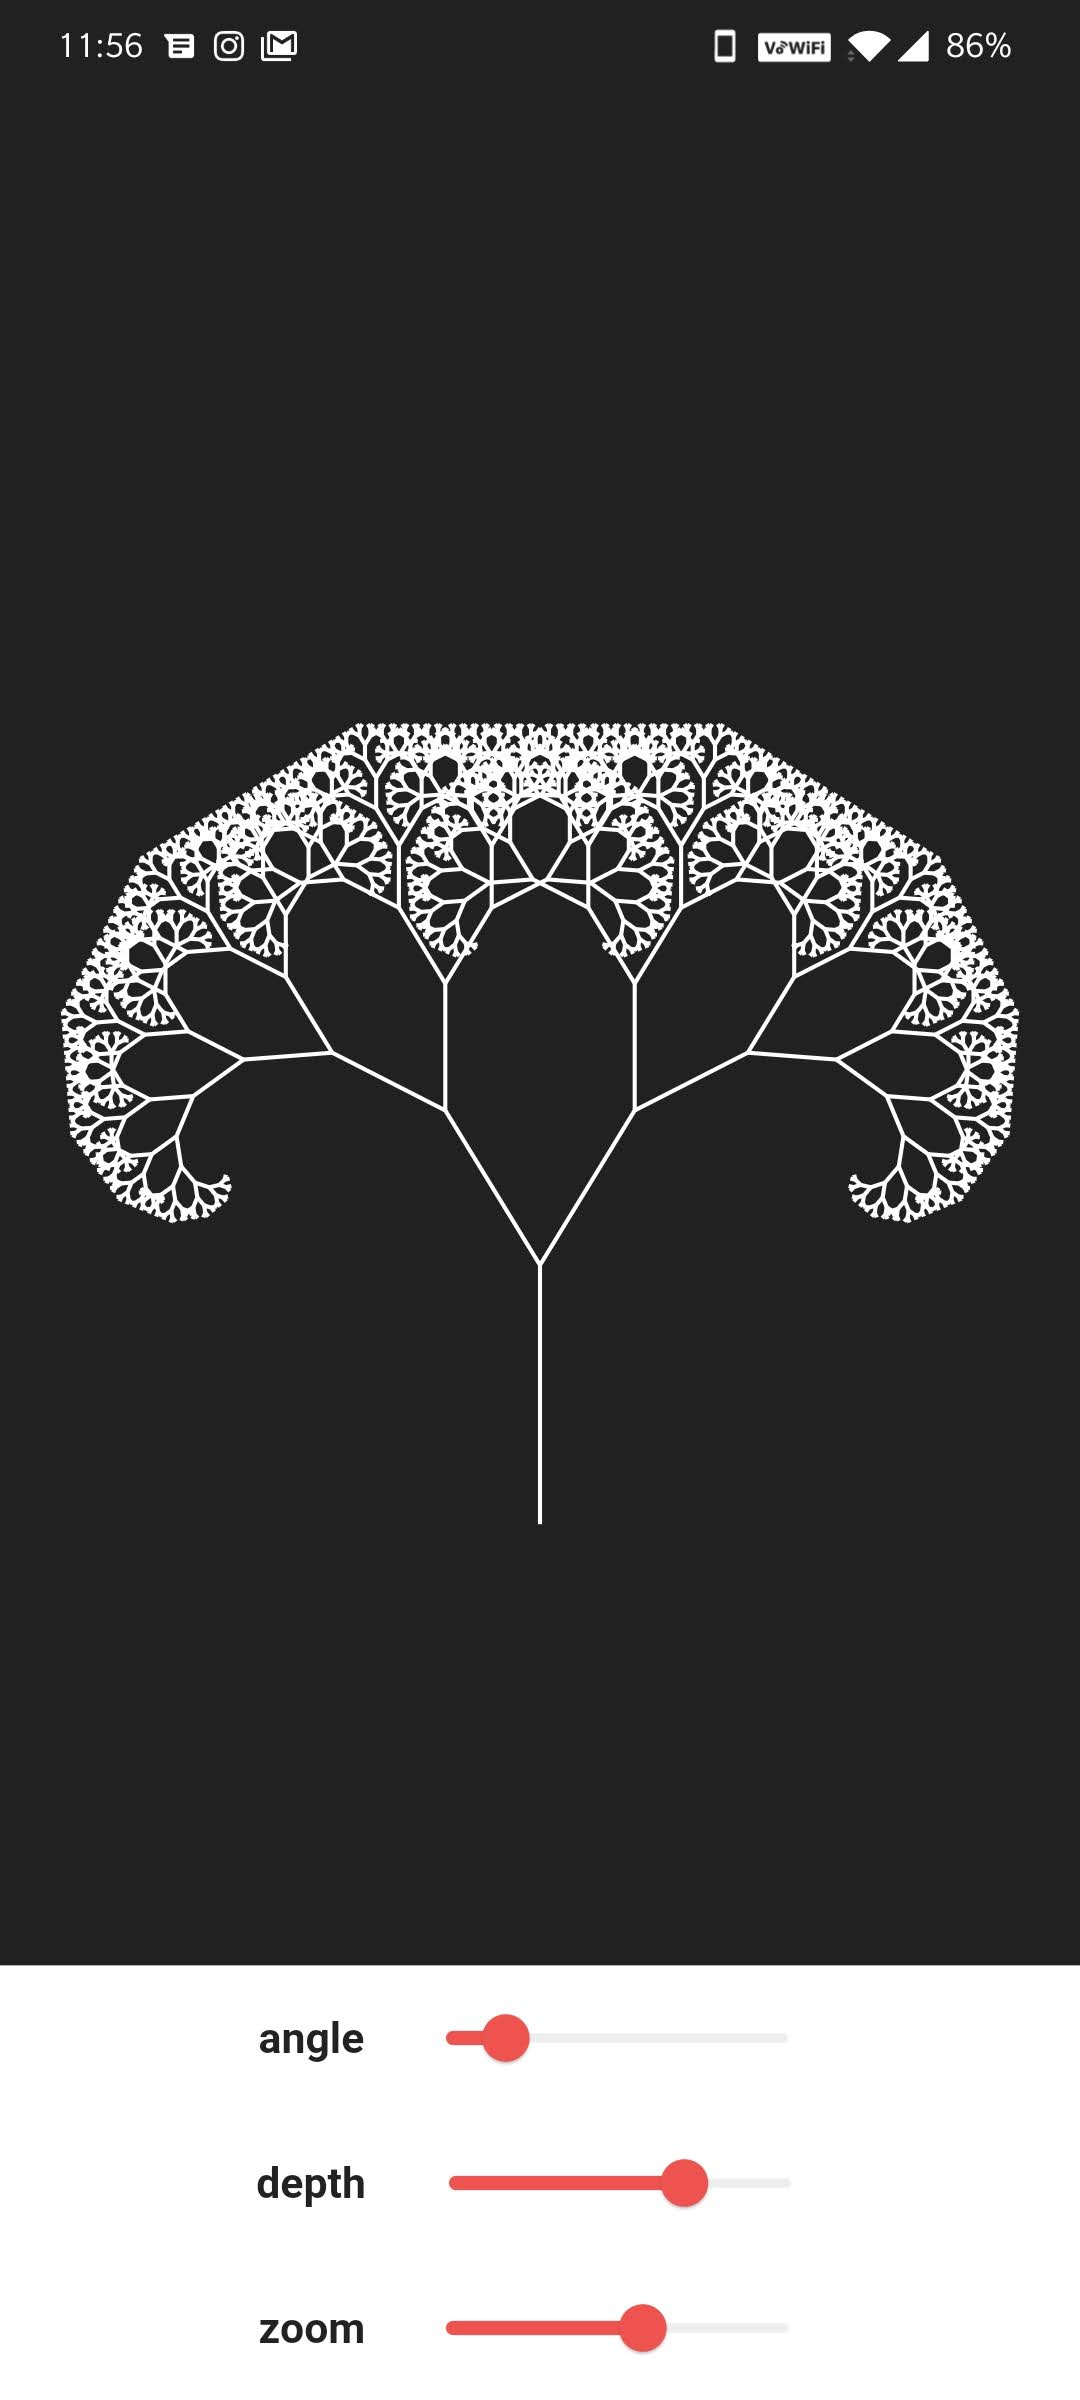
\includegraphics[width=3cm]{fractal_tree_ss_1}}

Conventional Statistics involve characterizing surfaces. This multiple scalar nature can be depicted through fractal geometry.\textsuperscript{[5]}

To have an even clearer view of the above, we have prepared a simulation for the same. Attached are some screenshots of the same.

In the given simulation, notice the sliders at the bottom. These represent the angle between branches, the depth of the tree, and the zoom level respectively. Even a slight change in the angle or the depth can produce an entirely different result.

Basically, the simulation of a Fractal Tree is a recursive function. It has 2 parameters:
\begin{itemize}
    \item \textbf{angle}
    \item \textbf{length}
\end{itemize}

The angle determines the angle of inclination between the current branch and its parent branch. The depth determines the depth of the tree (number of levels).

The length of the initial branch is directly proportional to the depth of the tree. After each level, the length of the branch reduces by 30\%. Thus, the bigger the depth, the denser the tree.

Here are some more screenshots:\\

\begin{figure}[h]
\hskip 3.27cm
\vspace{40pt}
\fbox{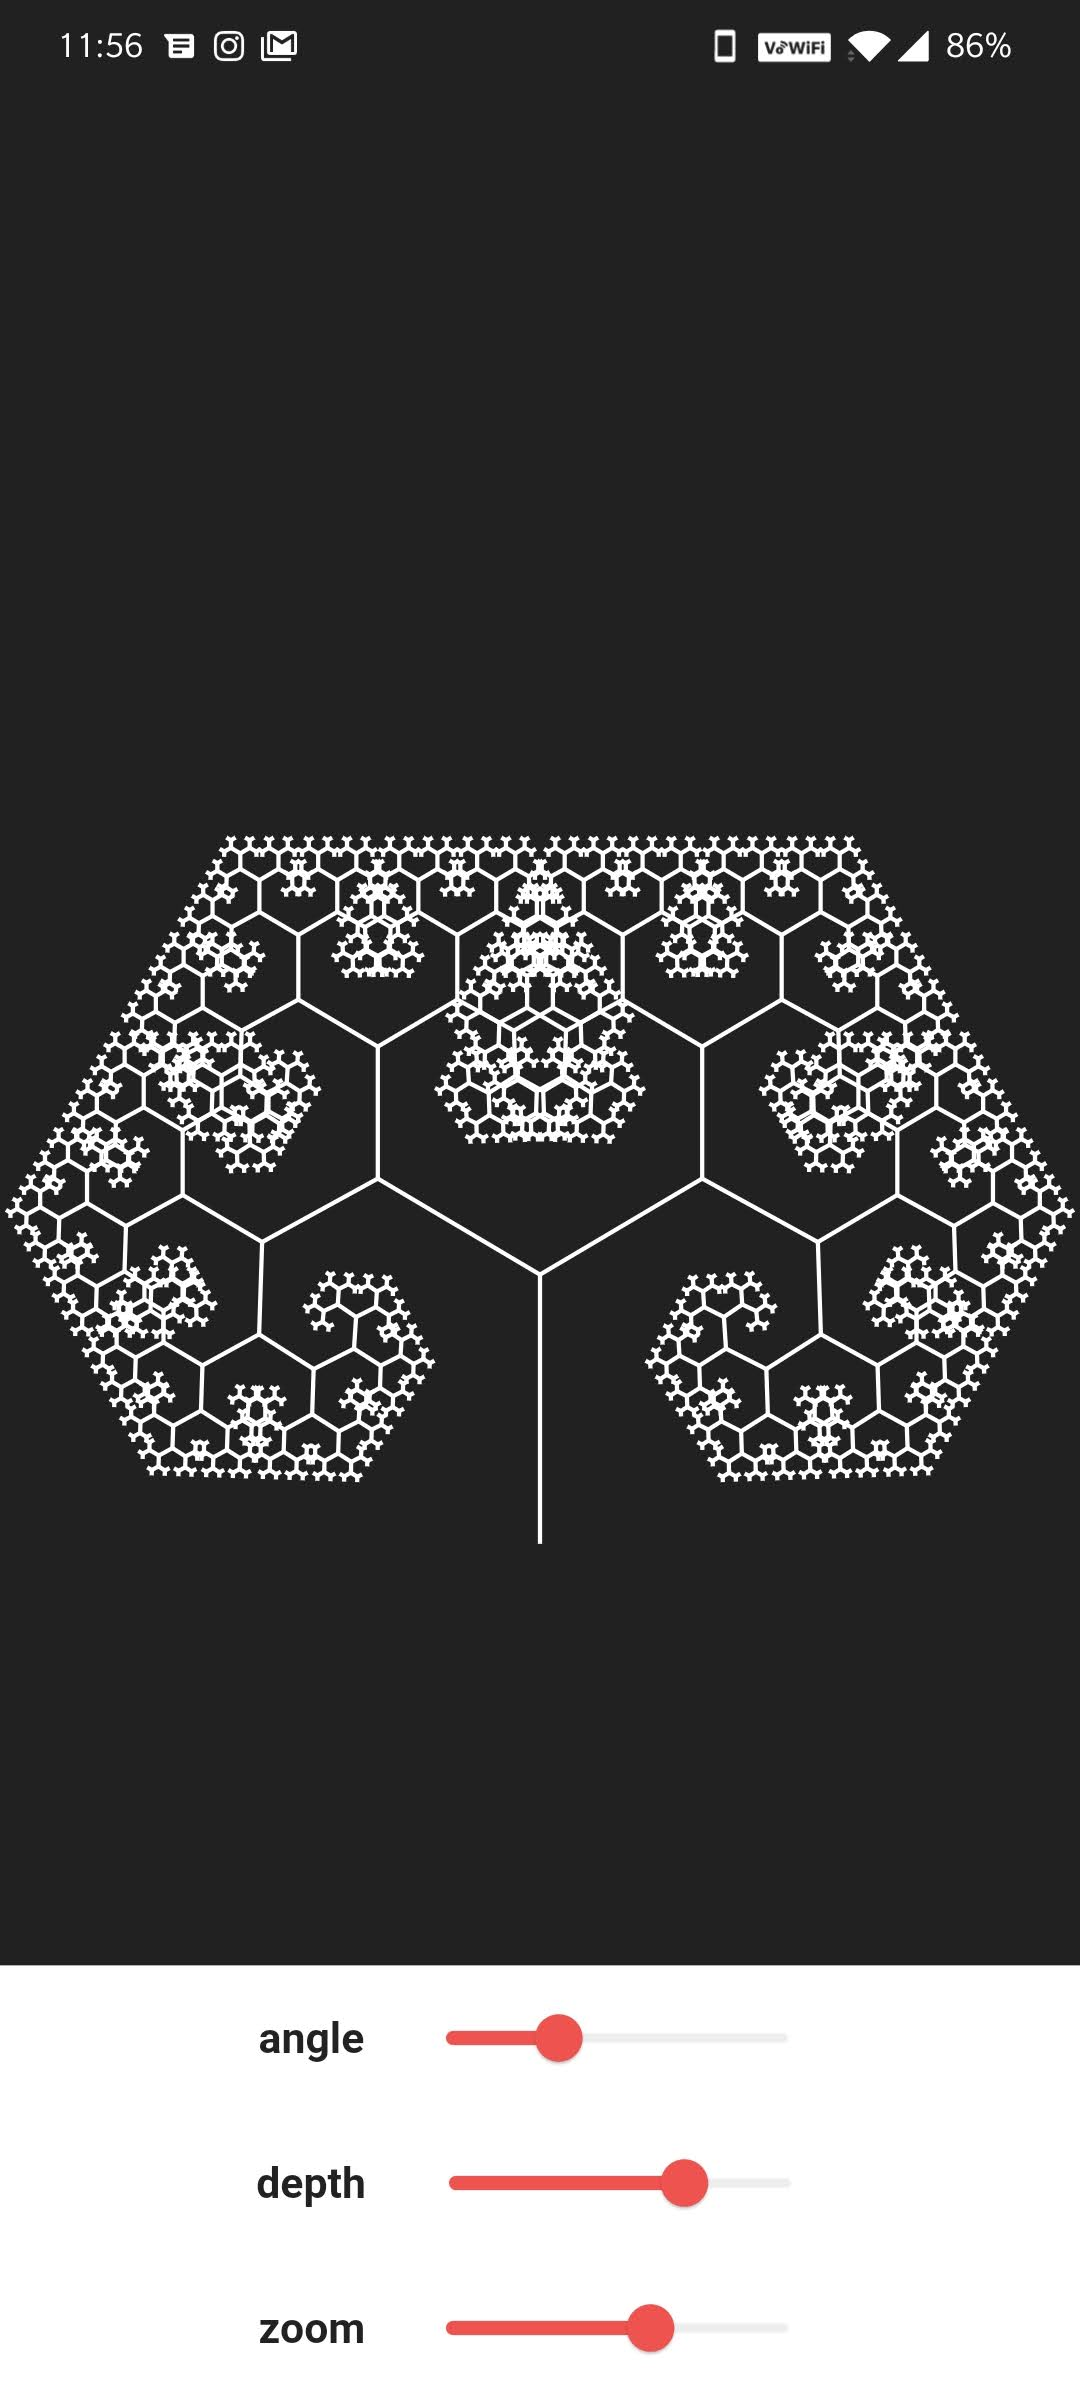
\includegraphics[width=3.3cm]{fractal_tree_ss_2}}
\fbox{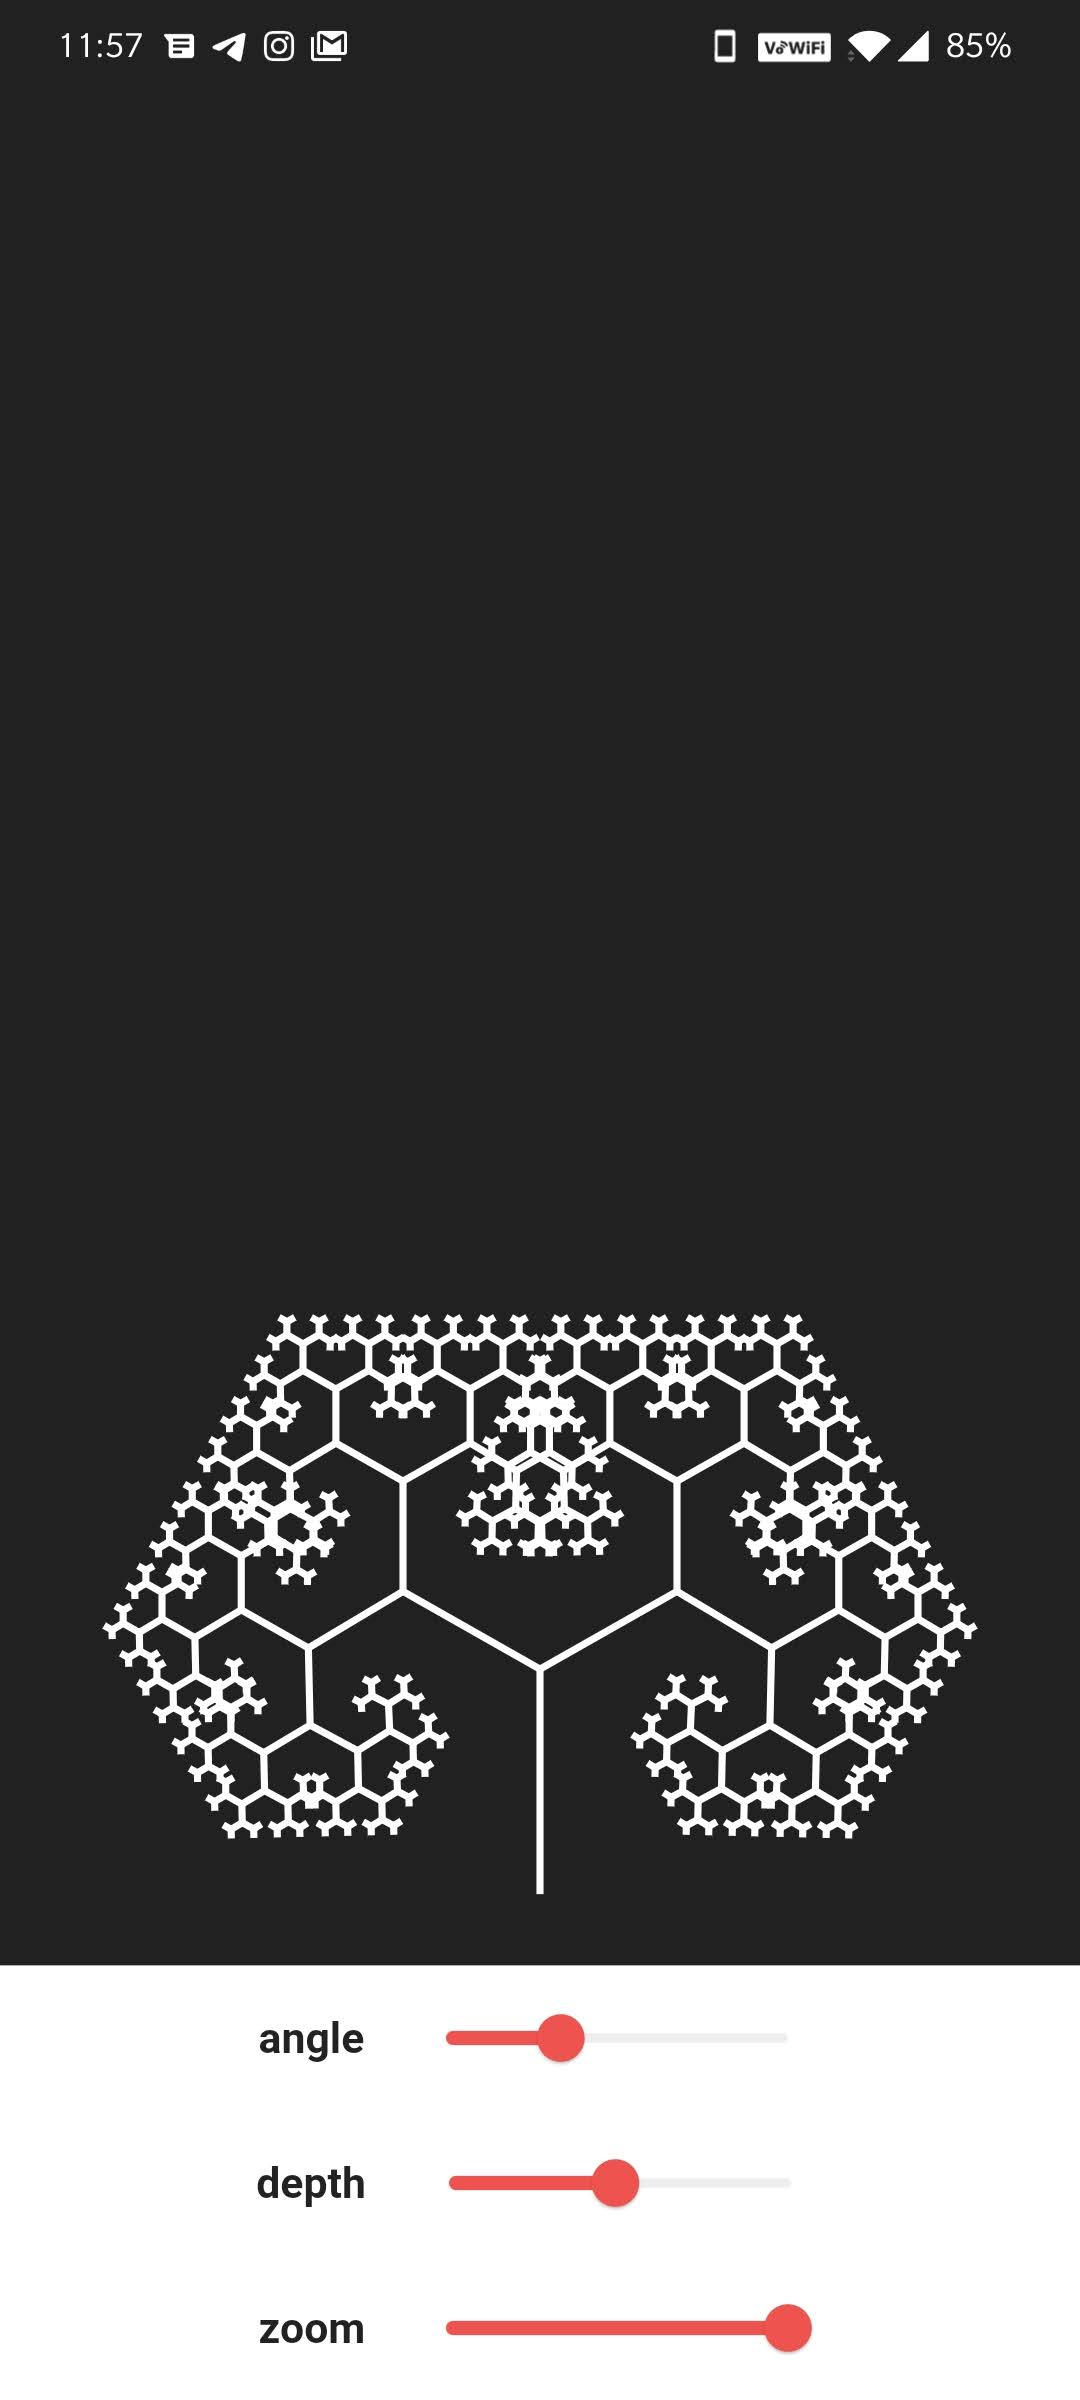
\includegraphics[width=3.3cm]{fractal_tree_ss_3}}
\end{figure}

\setlength{\leftskip}{-0cm}
Now, let's try making the tree as dense as possible.\\

\pagebreak
\begin{figure}[h]
    \vspace{10pt}
    \hskip -0.7cm
    \fbox{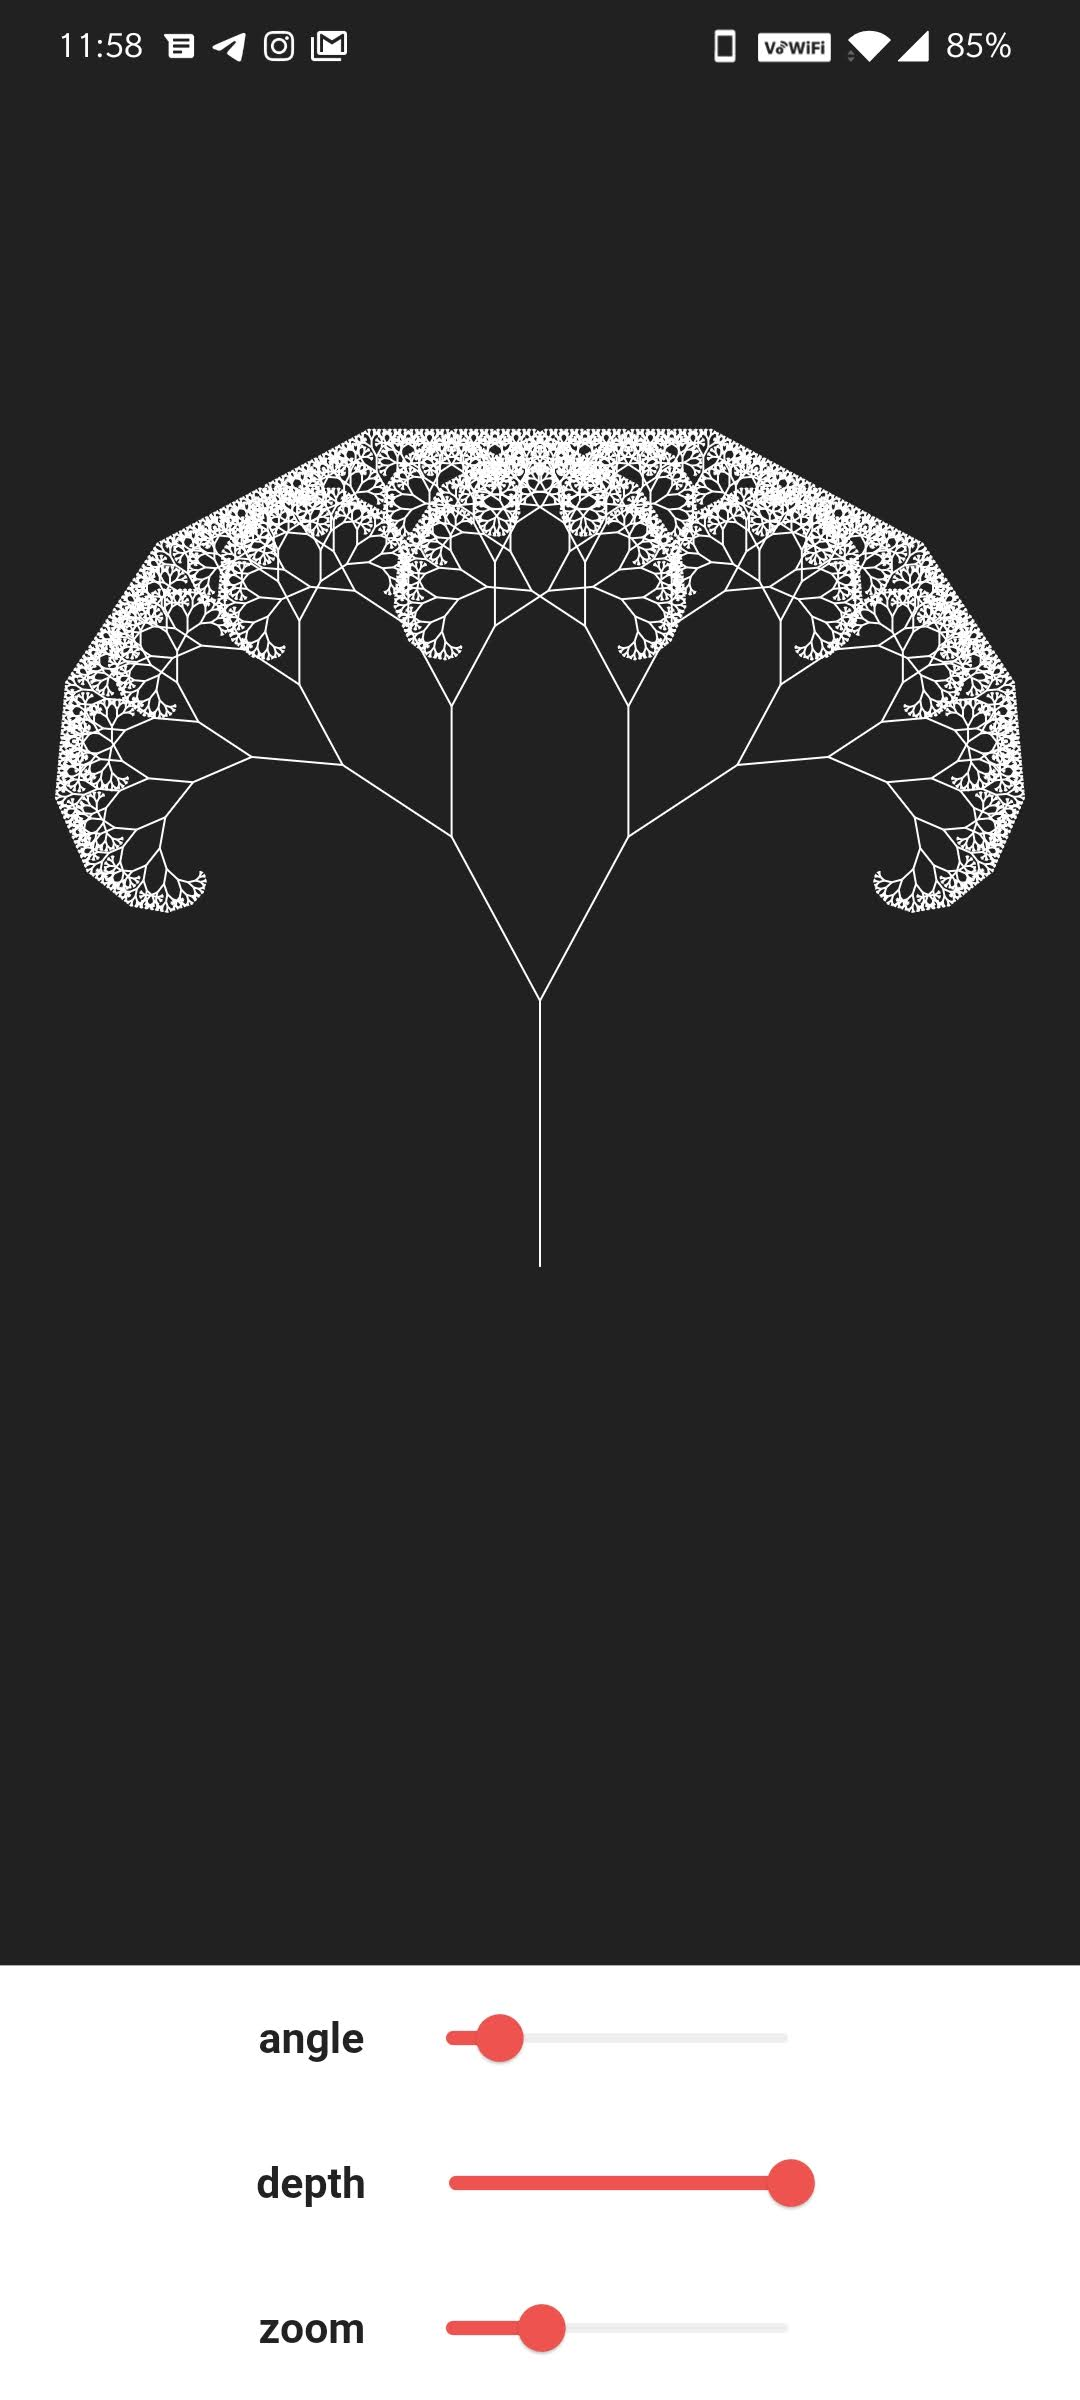
\includegraphics[width=3.3cm]{fractal_tree_ss_4}}
    \fbox{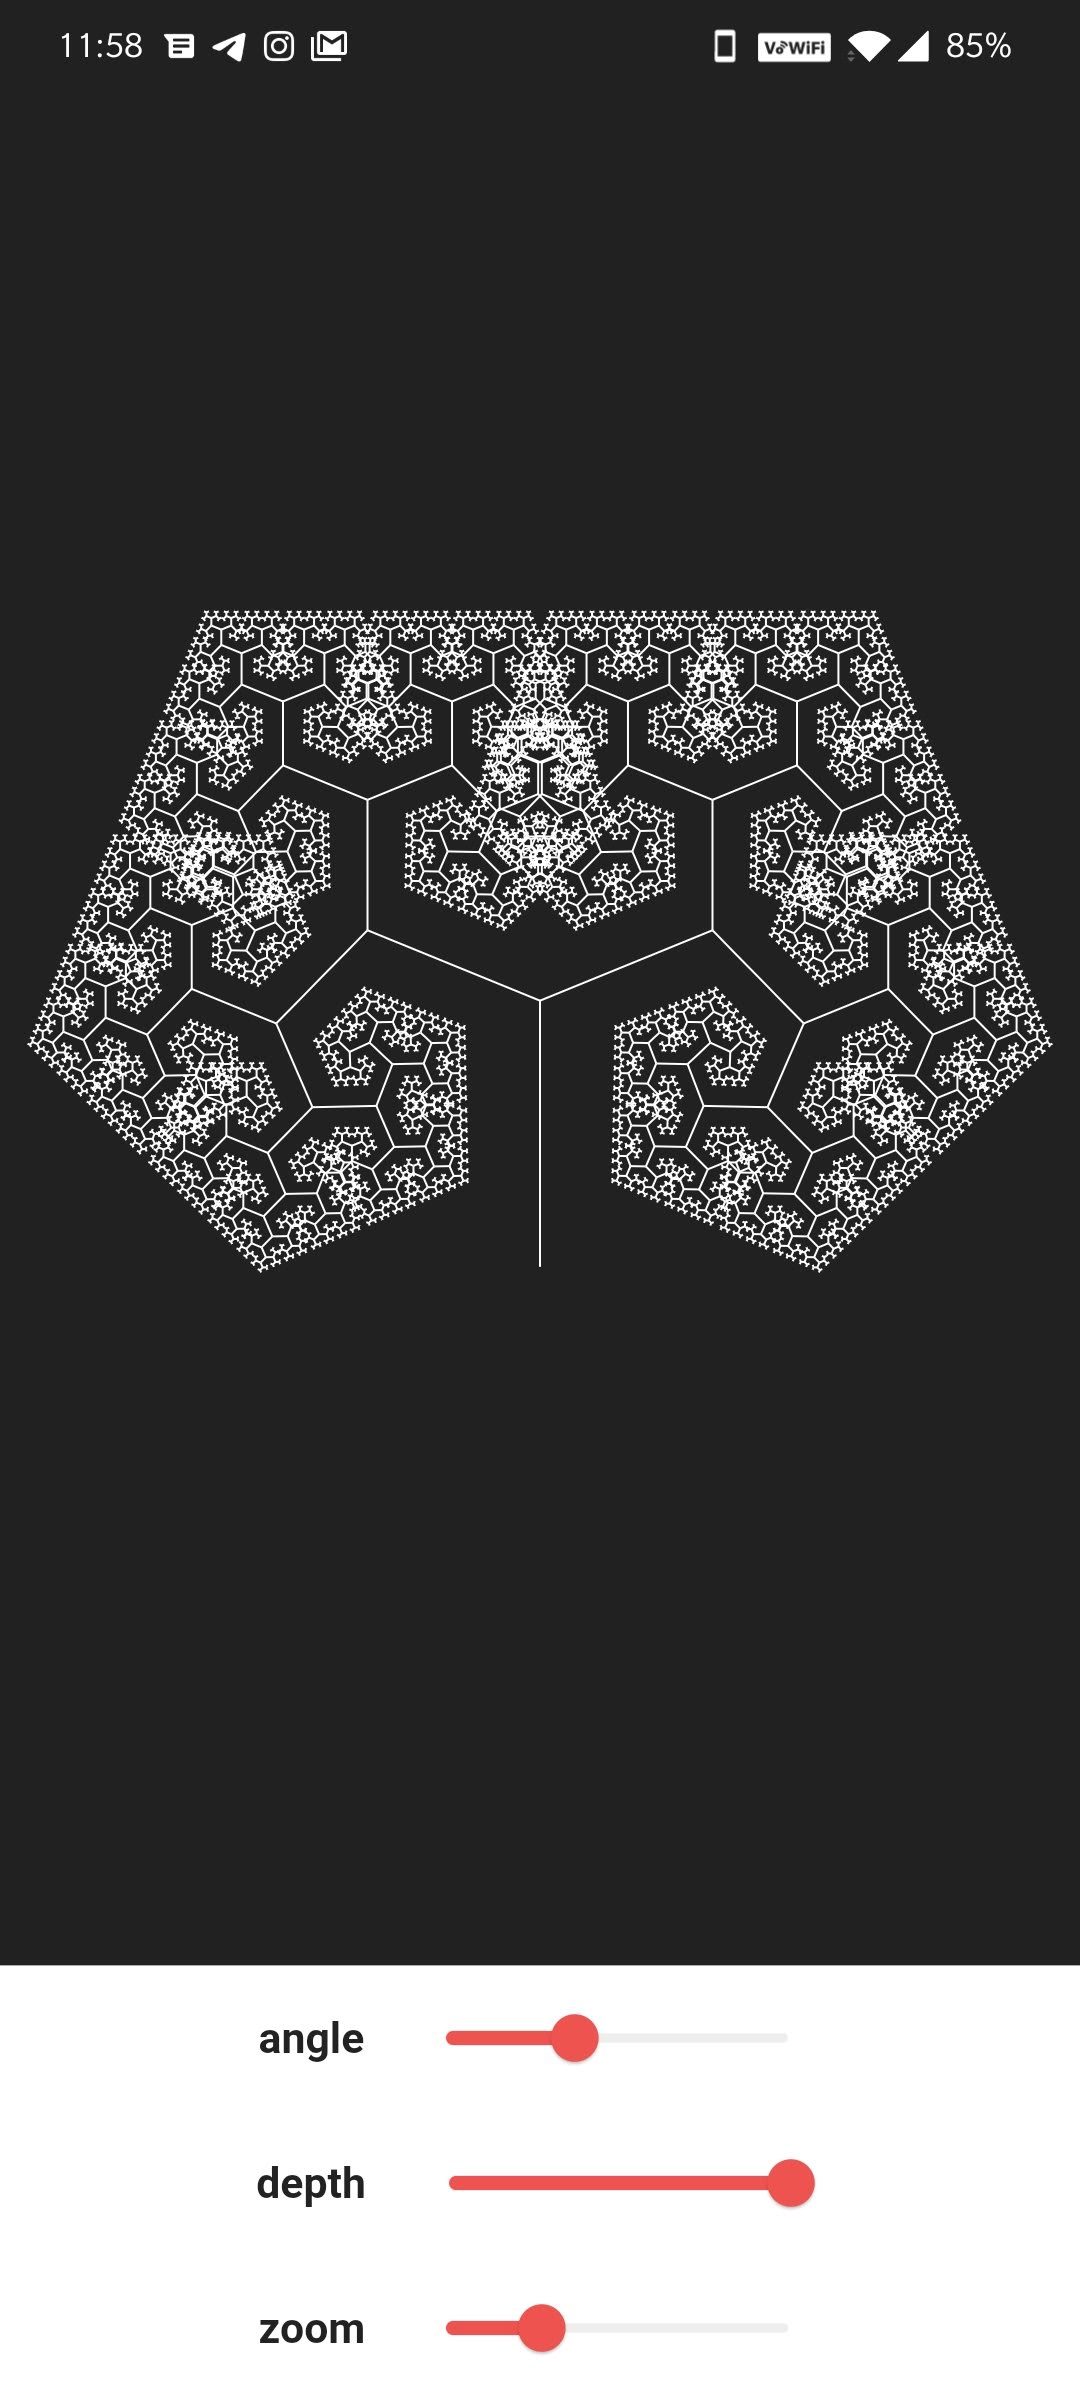
\includegraphics[width=3.3cm]{fractal_tree_ss_5}}
\end{figure}

The tree is a lot denser, and a lot taller now. Changing the angle makes the density difference look\leftHighlight{\textcolor{blue}{\url{https://bit.ly/fractals_simulation}}} even more profound. For reference, the video is hosted \textcolor{blue}{\href{https://bit.ly/fractals_simulation}{here}}.

\section{Estimation of Pi}

The plan is to simulate random \textbf{(x, y)} points on a 2-D plane with the domain as a square of side \textbf{2R} units. Consider a circle inside the same domain with the same diameter and inscribed into the square. Basically,

$$\frac{area\ of\ the\ circle}{area\ of\ the\ square}\ =\ \frac{number\ of\ points\ inside\ the\ circle}{total\ number\ of\ points\ generated}\ =\ \frac{\Pi r\textsuperscript{2}}{4r2}\ =\ \frac{\Pi}{4}\ =\ k$$

that is,

$$\Pi\ =\ 4\ *\ k$$

The points are generated in the \textbf{Dart} language using the \textit{dart:math} library, i.e.

$$x\ =\ rand(-R,\ R)$$
$$y\ =\ rand(-R,\ R)$$
$$where\ \textbf{rand(a,\ b)}\ generates\ random\ points\ between\ a\ and\ b$$

This is assuming that the centres of both, the square and the circle, lie at the \textbf{origin}.

\authorIntro{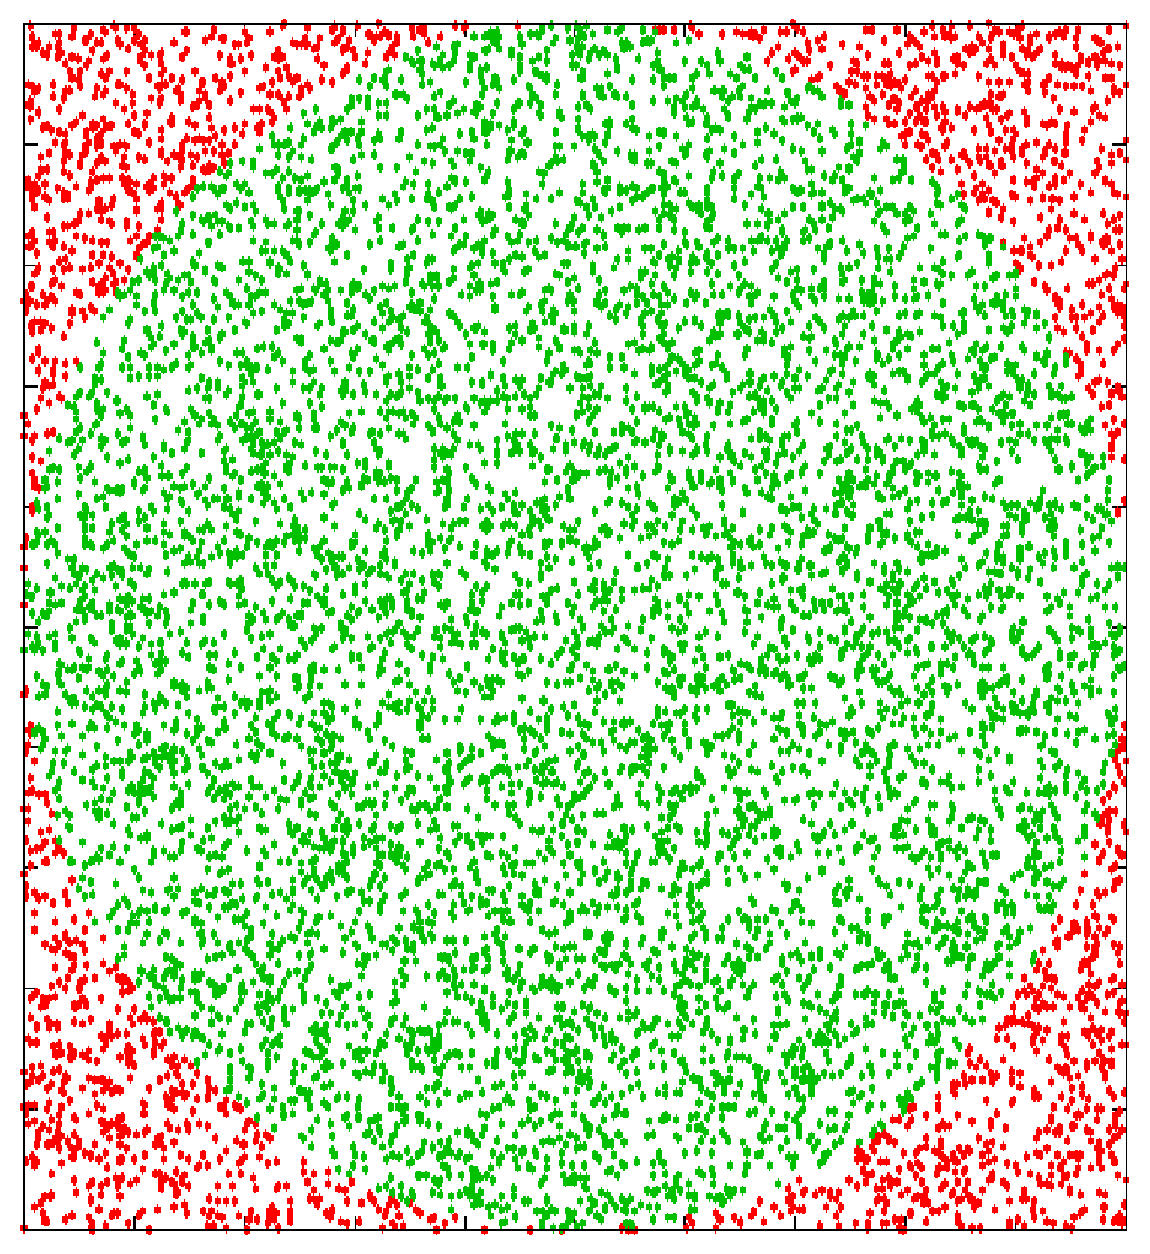
\includegraphics[width=3.5cm, height=3.5cm]{pi}\\
Source: \\
\textcolor{blue}{\url{www.physics.smu.edu}}}

Now that random points are generated, we start plotting them. If the generated point lies within the circle, we mark it with \textit{green}, else with \textit{red}. The value given by \textbf{4 * k} then evaluates to:

$$\Pi\ =\ 4\ *\ k\ =\ 4\ *\ \frac{number\ of\ green\ dots}{total\ number\ of\ dots\ (green\ +\ red)}$$

The best thing is that we don’t need to consider graphics for simulation. We only need to output random \textbf{(x, y)} pairs and then do the following:

\begin{itemize}
    \item if the point lies inside the circle - increment number of points inside the circle
    \item increment the total number of points irrespective of where the point lies
    \item calculate the above result, i.e. \textbf{4 * k}
\end{itemize}

To have a clearer view of the above, we have prepared a simulation for the same. Here are some screenshots of the same:

\pagebreak

\begin{figure}
    \hskip-3.5cm
    \vspace{20pt}
    \fbox{\includegraphics[width=4cm]{pi_ss_1}}
    \fbox{\includegraphics[width=4cm]{pi_ss_2}}
    \fbox{\includegraphics[width=4cm]{pi_ss_3}}
\end{figure}

In the above, it is clearly evident that as the number of points increases, the approximate value of Pi approaches the real value. This is in complete agreement with the hypotheses above, and hence, proves that Monte Carlo simulations are good approximations when one can’t calculate the exact value.

\leftHighlight{\textcolor{blue}{\url{https://bit.ly/pi_approximation}}}

The complete simulation video is available \textcolor{blue}{\href{https://bit.ly/pi_approximation}{here}}.

\section{Conclusion}
In this paper, Monte Carlo simulations have been used to show two test cases:
\begin{itemize}
\item simulating Fractal Trees, and
\item estimating the value of Pi
\end{itemize}

This method has been shown to be valid and effective, through testing at various parameters.


\begin{thebibliography}{99}

\bibitem{latexcompanion}
“A Gentle Introduction to Monte Carlo Sampling for Probability”\\ \textcolor{blue}{\url{https://machinelearningmastery.com/monte-carlo-sampling-for-probability/}}\\
{[Accessed: 7-April-2020]}\\

\bibitem{latexcompanion}
"Monte Carlo Simulations”\\ \textcolor{blue}{\url{https://www.palisade.com/risk/monte_carlo_simulation.asp}}\\
{[Accessed: 10-April-2020]}\\

\bibitem{latexcompanion}
"Mathematical Foundations of Monte Carlo Methods”\\ \textcolor{blue}{\url{https://www.scratchapixel.com/lessons/mathematics-physics-for-computer-graphics/monte-carlo-methods-mathematical-foundations/pdf-and-cdf}}\\
{[Accessed: 12-April-2020]}\\

\bibitem{latexcompanion}
"Monte Carlo Methods and Importance Sampling”\\ \textcolor{blue}{\url{http://ib.berkeley.edu/labs/slatkin/eriq/classes/guest\_lect/mc\_lecture\_notes.pdf }}\\
{[Accessed: 2-May-2020]}\\

\bibitem{latexcompanion}
Zou, Mingqing, et al. "A Monte Carlo method for simulating fractal surfaces." \textit{Physica A: Statistical Mechanics and its Applications} 386.1 (2007): 176-186.\\

\bibitem{latexcompanion}
Lin, Yi-Cheng, and Kamal Sarabandi. "A Monte Carlo coherent scattering model for forest canopies using fractal-generated trees." \textit{IEEE Transactions on Geoscience and Remote Sensing} 37.1 (1999): 440-451.\\

\bibitem{latexcompanion}
"Classification of Fractals”\\ \textcolor{blue}{\url{https://www.cs.mcgill.ca/~rwest/wikispeedia/wpcd/wp/f/Fractal.htm}}\\
{[Accessed: 28-May-2020]}\\

\bibitem{latexcompanion}
"General Introduction to Fractal Geometry”\\ \textcolor{blue}{\url{http://www.fractal.org/Bewustzijns-Besturings-Model/Fractals-Useful-Beauty.htm}}\\
{[Accessed: 31-May-2020]}\\

\bibitem{latexcompanion}
"Source of Fractals”\\ \textcolor{blue}{\url{http://www.fractal.org/Bewustzijns-Besturings-Model/Source-of-Fractals.htm}}\\
{[Accessed: 6-June-2020]}\\

\bibitem{latexcompanion}
Pippa, Natassa, et al. “On the Ubiquitous Presence of Fractals and Fractal Concepts in Pharmaceutical Sciences: A Review.” \textit{International Journal of Pharmaceutics}, Elsevier, 8 Sept. 2013,\\
\textcolor{blue}{\url{www.sciencedirect.com/science/article/pii/S0378517313008211}}

\end{thebibliography}

\end{document}


